% -*- Mode:TeX -*-

%% IMPORTANT: The official thesis specifications are available at:
%%            http://libraries.mit.edu/archives/thesis-specs/
%%
%%            Please verify your thesis' formatting and copyright
%%            assignment before submission.  If you notice any
%%            discrepancies between these templates and the 
%%            MIT Libraries' specs, please let us know
%%            by e-mailing thesis@mit.edu

%% The documentclass options along with the pagestyle can be used to generate
%% a technical report, a draft copy, or a regular thesis.  You may need to
%% re-specify the pagestyle after you \include  cover.tex.  For more
%% information, see the first few lines of mitthesis.cls. 

%\documentclass[12pt,vi,twoside]{mitthesis}
%%
%%  If you want your thesis copyright to you instead of MIT, use the
%%  ``vi'' option, as above.
%%
%\documentclass[12pt,twoside,leftblank]{mitthesis}
%%
%% If you want blank pages before new chapters to be labelled ``This
%% Page Intentionally Left Blank'', use the ``leftblank'' option, as
%% above. 

\documentclass[12pt,twoside]{mitthesis}
\usepackage{lgrind}
\usepackage{xcolor}
%% These have been added at the request of the MIT Libraries, because
%% some PDF conversions mess up the ligatures.  -LB, 1/22/2014
\usepackage{cmap}
\usepackage[T1]{fontenc}
\pagestyle{plain}

\newcommand{\TL}[1]{\textcolor{red}{Tzu-Mao: #1}}

%% My packages
\usepackage{amsmath}
\usepackage{amssymb}
\usepackage{graphicx}
\usepackage{hyperref}
\usepackage{caption}
\usepackage{subcaption}


%% This bit allows you to either specify only the files which you wish to
%% process, or `all' to process all files which you \include.
%% Krishna Sethuraman (1990).

% \typein [\files]{Enter file names to process, (chap1,chap2 ...), or `all' to
% process all files:}
% \def\all{all}
% \ifx\files\all \typeout{Including all files.} \else \typeout{Including only \files.} \includeonly{\files} \fi

\begin{document}

% -*-latex-*-
% 
% For questions, comments, concerns or complaints:
% thesis@mit.edu
% 
%
% $Log: cover.tex,v $
% Revision 1.8  2008/05/13 15:02:15  jdreed
% Degree month is June, not May.  Added note about prevdegrees.
% Arthur Smith's title updated
%
% Revision 1.7  2001/02/08 18:53:16  boojum
% changed some \newpages to \cleardoublepages
%
% Revision 1.6  1999/10/21 14:49:31  boojum
% changed comment referring to documentstyle
%
% Revision 1.5  1999/10/21 14:39:04  boojum
% *** empty log message ***
%
% Revision 1.4  1997/04/18  17:54:10  othomas
% added page numbers on abstract and cover, and made 1 abstract
% page the default rather than 2.  (anne hunter tells me this
% is the new institute standard.)
%
% Revision 1.4  1997/04/18  17:54:10  othomas
% added page numbers on abstract and cover, and made 1 abstract
% page the default rather than 2.  (anne hunter tells me this
% is the new institute standard.)
%
% Revision 1.3  93/05/17  17:06:29  starflt
% Added acknowledgements section (suggested by tompalka)
% 
% Revision 1.2  92/04/22  13:13:13  epeisach
% Fixes for 1991 course 6 requirements
% Phrase "and to grant others the right to do so" has been added to 
% permission clause
% Second copy of abstract is not counted as separate pages so numbering works
% out
% 
% Revision 1.1  92/04/22  13:08:20  epeisach

% NOTE:
% These templates make an effort to conform to the MIT Thesis specifications,
% however the specifications can change.  We recommend that you verify the
% layout of your title page with your thesis advisor and/or the MIT 
% Libraries before printing your final copy.
\title{Learning non-stationary SVBRDFs using GANs and Differentiable Rendering}

\author{Budmonde Duinkharjav}
% If you wish to list your previous degrees on the cover page, use the 
% previous degrees command:
% You can use the \\ command to list multiple previous degrees
%       \prevdegrees{B.S., University of California (1978) \\
%                    S.M., Massachusetts Institute of Technology (1981)}
\prevdegrees{B.S., Massachusetts Institute of Technology (2018)}
\department{Department of Electrical Engineering and Computer Science}

% If the thesis is for two degrees simultaneously, list them both
% separated by \and like this:
% \degree{Doctor of Philosophy \and Master of Science}
\degree{Master of Engineering in Computer Science and Engineering}

% As of the 2007-08 academic year, valid degree months are September, 
% February, or June.  The default is June.
\degreemonth{June}
\degreeyear{2019}
\thesisdate{May 24, 2019}

%% By default, the thesis will be copyrighted to MIT.  If you need to copyright
%% the thesis to yourself, just specify the `vi' documentclass option.  If for
%% some reason you want to exactly specify the copyright notice text, you can
%% use the \copyrightnoticetext command.  
%\copyrightnoticetext{\copyright IBM, 1990.  Do not open till Xmas.}

% If there is more than one supervisor, use the \supervisor command
% once for each.
\supervisor{Fr\'edo Durand}{Professor of Electrical Engineering and Computer Science}

% This is the department committee chairman, not the thesis committee
% chairman.  You should replace this with your Department's Committee
% Chairman.
\chairman{Katrina LaCurts}{Chairman, Department Committee on Graduate Theses}

% Make the titlepage based on the above information.  If you need
% something special and can't use the standard form, you can specify
% the exact text of the titlepage yourself.  Put it in a titlepage
% environment and leave blank lines where you want vertical space.
% The spaces will be adjusted to fill the entire page.  The dotted
% lines for the signatures are made with the \signature command.
\maketitle

% The abstractpage environment sets up everything on the page except
% the text itself.  The title and other header material are put at the
% top of the page, and the supervisors are listed at the bottom.  A
% new page is begun both before and after.  Of course, an abstract may
% be more than one page itself.  If you need more control over the
% format of the page, you can use the abstract environment, which puts
% the word "Abstract" at the beginning and single spaces its text.

%% You can either \input (*not* \include) your abstract file, or you can put
%% the text of the abstract directly between the \begin{abstractpage} and
%% \end{abstractpage} commands.

% First copy: start a new page, and save the page number.
\cleardoublepage
% Uncomment the next line if you do NOT want a page number on your
% abstract and acknowledgments pages.
% \pagestyle{empty}
\setcounter{savepage}{\thepage}
\begin{abstractpage}
In this thesis we propose a learning approach for generating realistic SVBRDFs
using generative adversarial models and differentiable rendering. Our model
learns a mapping from the \emph{geometry buffer} of a surface to a corresponding
albedo texture-map by training on images of the same surface rendered using a
target texture-map. A key feature of this learning process is the ability to
differentiate the render function within our model; this enables the optimization
of the texture-map generator parameters using a loss function computed from the
rendered 2D images. Our results show that differentiable rendering is applicable
in complex neural network models such as GANs, opening up opportunities for more
applications of deep learning methods in the computer graphics pipeline.
\end{abstractpage}

% Additional copy: start a new page, and reset the page number.  This way,
% the second copy of the abstract is not counted as separate pages.
% Uncomment the next 6 lines if you need two copies of the abstract
% page.
% \setcounter{page}{\thesavepage}
% \begin{abstractpage}
% In this thesis we propose a learning approach for generating realistic SVBRDFs
using generative adversarial models and differentiable rendering. Our model
learns a mapping from the \emph{geometry buffer} of a surface to a corresponding
albedo texture-map by training on images of the same surface rendered using a
target texture-map. A key feature of this learning process is the ability to
differentiate the render function within our model; this enables the optimization
of the texture-map generator parameters using a loss function computed from the
rendered 2D images. Our results show that differentiable rendering is applicable
in complex neural network models such as GANs, opening up opportunities for more
applications of deep learning methods in the computer graphics pipeline.
% \end{abstractpage}

\cleardoublepage

\section*{Acknowledgments}

Professor Fr\'edo Durand and Dr.\ Jun-Yan Zhu for their great guidance and mentorship
throughout my thesis project.

Dr.\ Tzu-Mao Li for providing general direction and feedback for my thesis project,
tutoring me in the research process, and heping me debug my code in numerous occasions.

Spandan Madan, Helen Ho, and Nishchal Bhandari, for their work on CoSy which allowed
me to bootstrap my project codebase and necessary data.

Everyone in the Computer Graphics Group, for tutoring me in my research experience and
providing useful feedback.

Toyota for providing funding for this research opportunity.

Tuul Damba-Ochir and Sophia Kwon, for collecting data for my project, proof-reading my
thesis write-up, and providing moral support.

% Some departments (e.g. 5) require an additional signature page.  See
% signature.tex for more information and uncomment the following line if
% applicable.
% \include{signature}
\pagestyle{plain}
  % -*- Mode:TeX -*-
%% This file simply contains the commands that actually generate the table of
%% contents and lists of figures and tables.  You can omit any or all of
%% these files by simply taking out the appropriate command.  For more
%% information on these files, see appendix C.3.3 of the LaTeX manual. 
\tableofcontents
\newpage
\listoffigures




\chapter{Introduction}

Fidelity of images produced by rendering pipelines is largely affected by the surface
reflectance model used in the rendering process. Physically based reflectance models used in
modern ray tracing engines help achieve a high level of realism. However, materials encountered
on real surfaces are rarely uniform and feature spatially-varying reflectances due to natural
causes such as wear and tear, weathering, and other surface imperfections. Unfortunately, using
procedural techniques to replicate the complexity of real spatially-varying materials largely
relies on handcrafted heuristics which produce results that are subjective in terms of realism.
To record the complexity of real materials, previous
methods~\cite{aittala2016reflectance, aittala2013practical, aittala2015two, deschaintre2018single}
use real photographs of simple flat surfaces to extract spatially-varying bidirectional
reflectance distribution functions (SVBRDFs). However, extracting the SVBRDF for more complex
surfaces with variable curvatures, such as dirt textures on car hulls, is a significantly harder
task not attempted by these methods not only due to the complexity of the surface geometry, but
also because of the non-stationary nature of the SVBRDFs; different areas of the surface would
experience different amounts of weathering, causing the resultant SVBRDF to not exhibit shift
invariance.

Exemplar based synthesis of complex textures is also studied in computer vision applications.
The advent of the GAN~\cite{goodfellow2014generative} paved the way for high fidelity results from
neural network based generative models for texture synthesis and style
transfer~\cite{zhu2017unpaired, isola2017image, zhou2018non}. Unfortunately, the deep learning
approach requires that a model's building blocks consist of differentiable functions. Since
differentiating more complex functions is often impractical, the majority of neural network models
use simple functions with explicit analytical derivatives. However, if we have methods for
differentiating complex functions, we enable opportunities to utilize deep learning methods in
more complex tasks.

Recent work by Li et al.~\cite{li2018differentiable} features a differentiable ray tracer which
makes it possible to take derivatives of images produced by the ray tracer with respect to the
scene description parameters such as surface vertices, material properties, camera parameters,
etc. The ability to take derivatives with respect to scene variables allows us to incorporate the
ray tracing function into deep learning methods to train complex neural network models for
generating surface geometry and textures.

In this thesis we demonstrate an application of a deep learning model for computer graphics
by training a neural network which incorporates the differentiable ray
tracer~\cite{li2018differentiable}. Specifically, we propose and implement a GAN that synthesizes
SVBRDFs of complex surfaces (like a car hull) using a dataset of 2D images of the surfaces. Our model
takes advantage of the differentiable ray tracer to compute a loss on a rendered image and
back-propagate it to train a generator network which synthesizes a realistic albedo texture-map for a
given 3D shape. We leave the synthesis of more complex SVBRDFs featuring specular reflectance,
glossiness, and normal maps as future work.

We present our results when trained on a synthetic dataset. Our dataset consists of rendered images
of car models with a target texture-map generated by a procedural surface weathering texture model
used commonly in computer graphics applications~\cite{bhandari2018procedural}. Unfortunately, for
the scope of this thesis, we are not able to extend our model to successfully learn texture-maps
from real images.
\chapter{Related Work}

\section{Texture synthesis and style transfer}

Our task shares similarities with texture synthesis and style transfer. In both tasks, the
objective is to separate the information describing \emph{what} the scene is from \emph{how}
it was depicted -- what style the scene was created in. E.g. a dataset of paintings of
architecture depicts some architectural scenery stylized as paintings. Texture synthesis
focuses on extracting the style of an image while style transfer focuses on morphing the
style of a scene. However, these tasks are ill-posed as the distinction between a scene and
its style is not well defined. Some work in the literature acknowledge this limitation and
propose methods that incorporate the distinction as part of the
problem~\cite{isola2017image, zhu2017unpaired} while others use perceptual judgment to
optimize for the best
results~\cite{gatys2015texture, gatys2016image, ulyanov2016texture, johnson2016perceptual}.
Other solutions assume the input image contains only style content and attempt to produce
similar images of the given texture \cite{wei2009sae, sendik2017deep, zhou2018non}. 

Fortunately, in our case, the distinction between the scene and style is concretely defined;
the scene is specified by the surface geometry, while the style is defined by the shading
materials used in the rendering pipeline.

The state-of-the-art approach for the task of texture-synthesis and style-transfer is to
train a Generative Adversarial Network~\cite{goodfellow2014generative} that generates the
desired output~\cite{johnson2016perceptual, isola2017image, zhu2017unpaired, zhou2018non}.
We base our network architecture from the CycleGAN model by Zhu et al.~\cite{zhu2017unpaired}.

\section{Physically-based appearance modeling}

Work in appearance modeling use the geometry of the models to simulate physical phenomena, such
as erosion of terrains~\cite{musgrave1989eroded}, chemical diffusion~\cite{turk1991diffusion},
metallic patinas~\cite{dorsey1996patinas}, wet materials~\cite{jensen1999wet}, weathering
(e.g.~\cite{dorsey1999weather, chen2005weathering, bosch2011weathering}). These methods
generate convincing materials from geometry, but need to use dedicated simulation methods for
different scenarios. In contrast our method is fully data-driven and does not rely on knowing
the physics of the materials. Combining two approaches remain an interesting research avenue.

Some other methods assume flat geometry, but use a more elaborate material model
(e.g.~\cite{barron2015sir, aittala2015two, deschaintre2018single}). These methods deliver
high-quality textures but do not take geometry into consideration.

\section{Deep learning models for computer graphics}

Applications of deep learning models in computer graphics literature is hindered due to the
complex operations used in the graphics pipeline. Specifically, using 2D rendered images to
infer an underlying 3D scene geometry relies on differentiating the rendering function.
A generative model with a differentiable renderer makes it possible to optimize the model
parameters using a loss function computed from a rendered image of a 3D scene which contains
the generator output. 

A variety of methods propose models for indirectly differentiating the rendering function
by optimizing a neural network to emulate
it~\cite{kulkarni2015deep, nguyen2018rendernet, nguyen2019hologan}. Others propose
differentiable rasterization algorithms tailored for their use
case~\cite{genova2018unsupervised, liu2019soft}. To our best knowledge, there is no prior
work in generative deep learning models featuring a general purpose ray tracer.

Our method incorporates the differentiable ray tracer by Li et
al.~\cite{li2018differentiable} into our model. This ray tracer is able to compute
derivatives of the Monte-Carlo path tracing algorithm for arbitrary scenes with surfaces
represented as triangle-meshes with respect to any scene parameters such as triangle-mesh
vertices, shading materials, and camera poses. The advantage of using this ray tracer over
others is that we are able to extract any desired scene variable explicitly which is useful
in most practical applications.

\chapter{Method} \label{ch:method}

We take on the following task: given a dataset of images of weathered cars,
learn a model that generates materials to approximate the appearance of
weathering on a car surface. We focus on Lambertian materials in this thesis and represent the material with a
semi-transparent albedo texture-map in the UV-embedding of the surface.

\begin{figure}[ht]
    \centering
    \caption{Our model pipeline takes as input a scene description $\Phi$ which contains:
        shape geometry, shading materials, camera parameters, and lighting parameters.
        The UV-embedding of the car triangle-mesh, allows us to extract the \emph{position}
        and \emph{normal} maps of the car in its UV-coordinates, which we refer to as the
        \emph{geometry buffer}. The \emph{geometry buffer} is used to generate the albedo
        of the dirt using our generator network $\mathcal{G}$. To produce the final render,
        we use a differentiable ray tracer $\mathcal{R}$ after compositing the dirt albedo
        onto the original shading material.}
    \label{fig:generator-pipeline}
    \vspace{0.2in}
    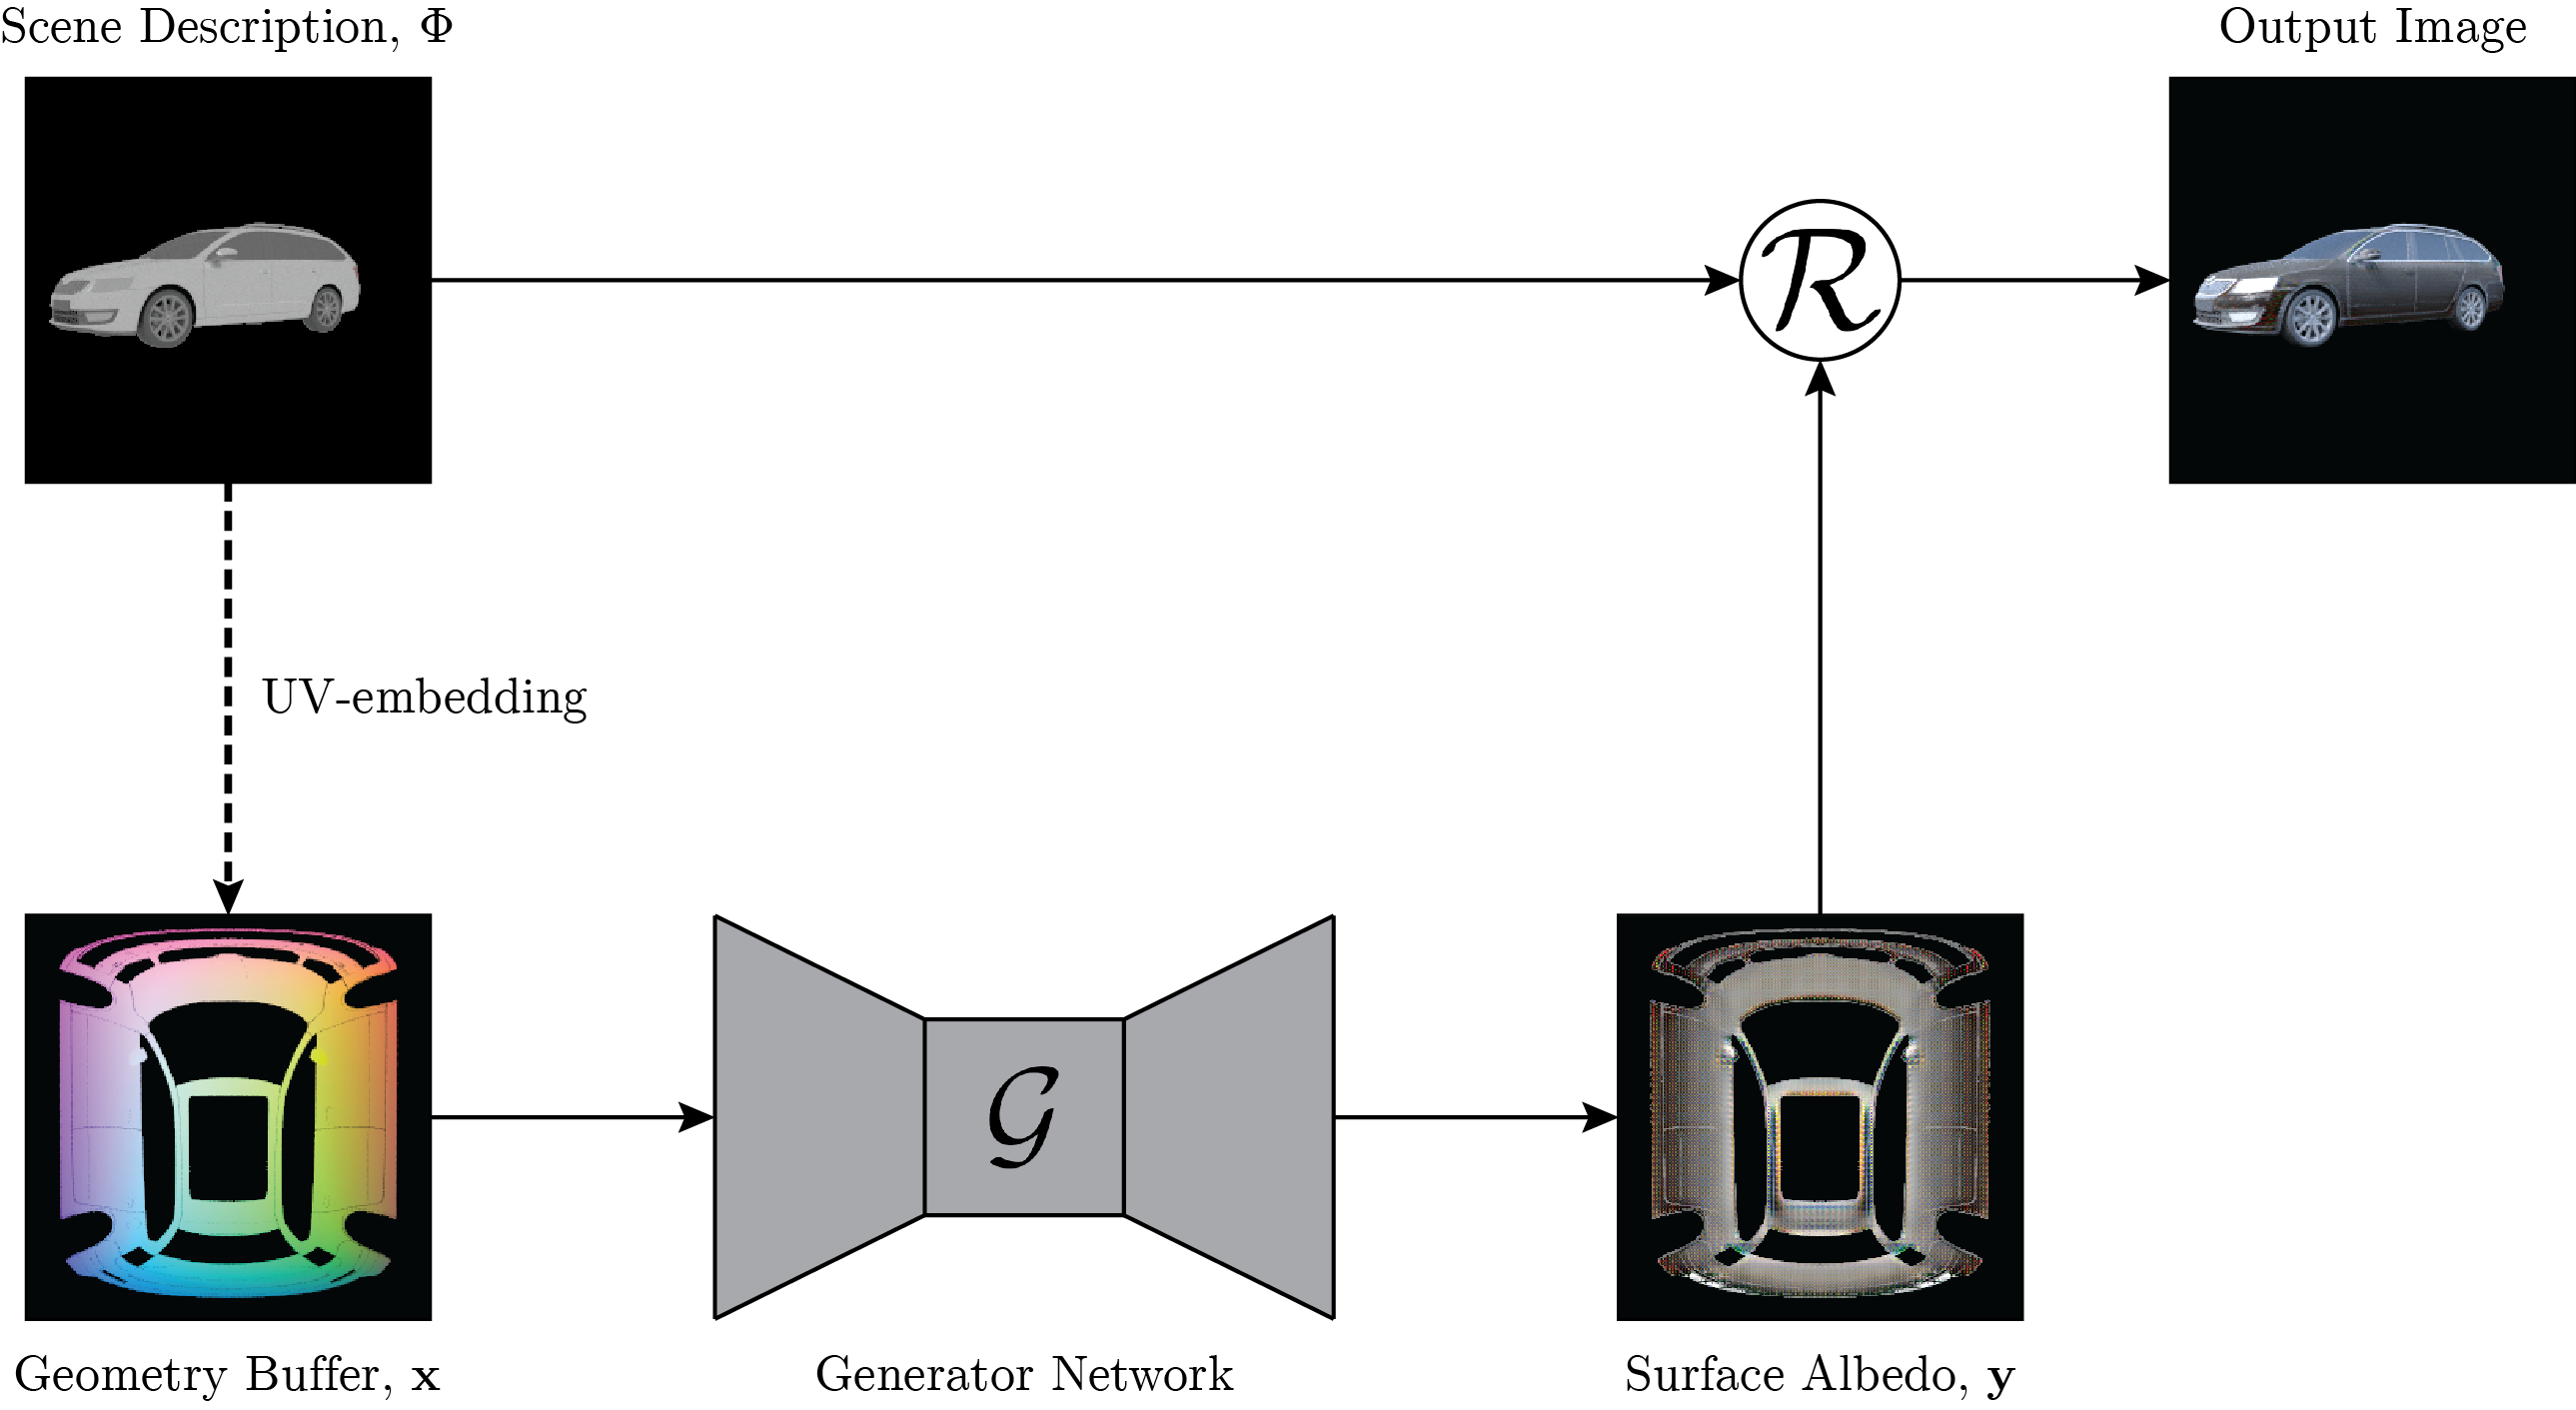
\includegraphics[width=.9\linewidth]{graphics/pipeline.png}
\end{figure}
\begin{figure}[ht]
    \centering
    \caption{We use a GAN training procedure for our model. In addition to our generator model $\mathcal{G}$, we
    train a discriminator model $\mathcal{D}$ that learns to discriminate whether an image was produced by the
    generator (fake) or was sampled from the dataset (real). The discriminator produces a down-sampled grid of
    the input image, with each pixel representing the likelihood of the input being real or fake. In the
    visualization below, the correspondence is: yellow -- real, cyan -- fake.}
    \label{fig:discriminator-pipeline}
    \vspace{0.2in}
    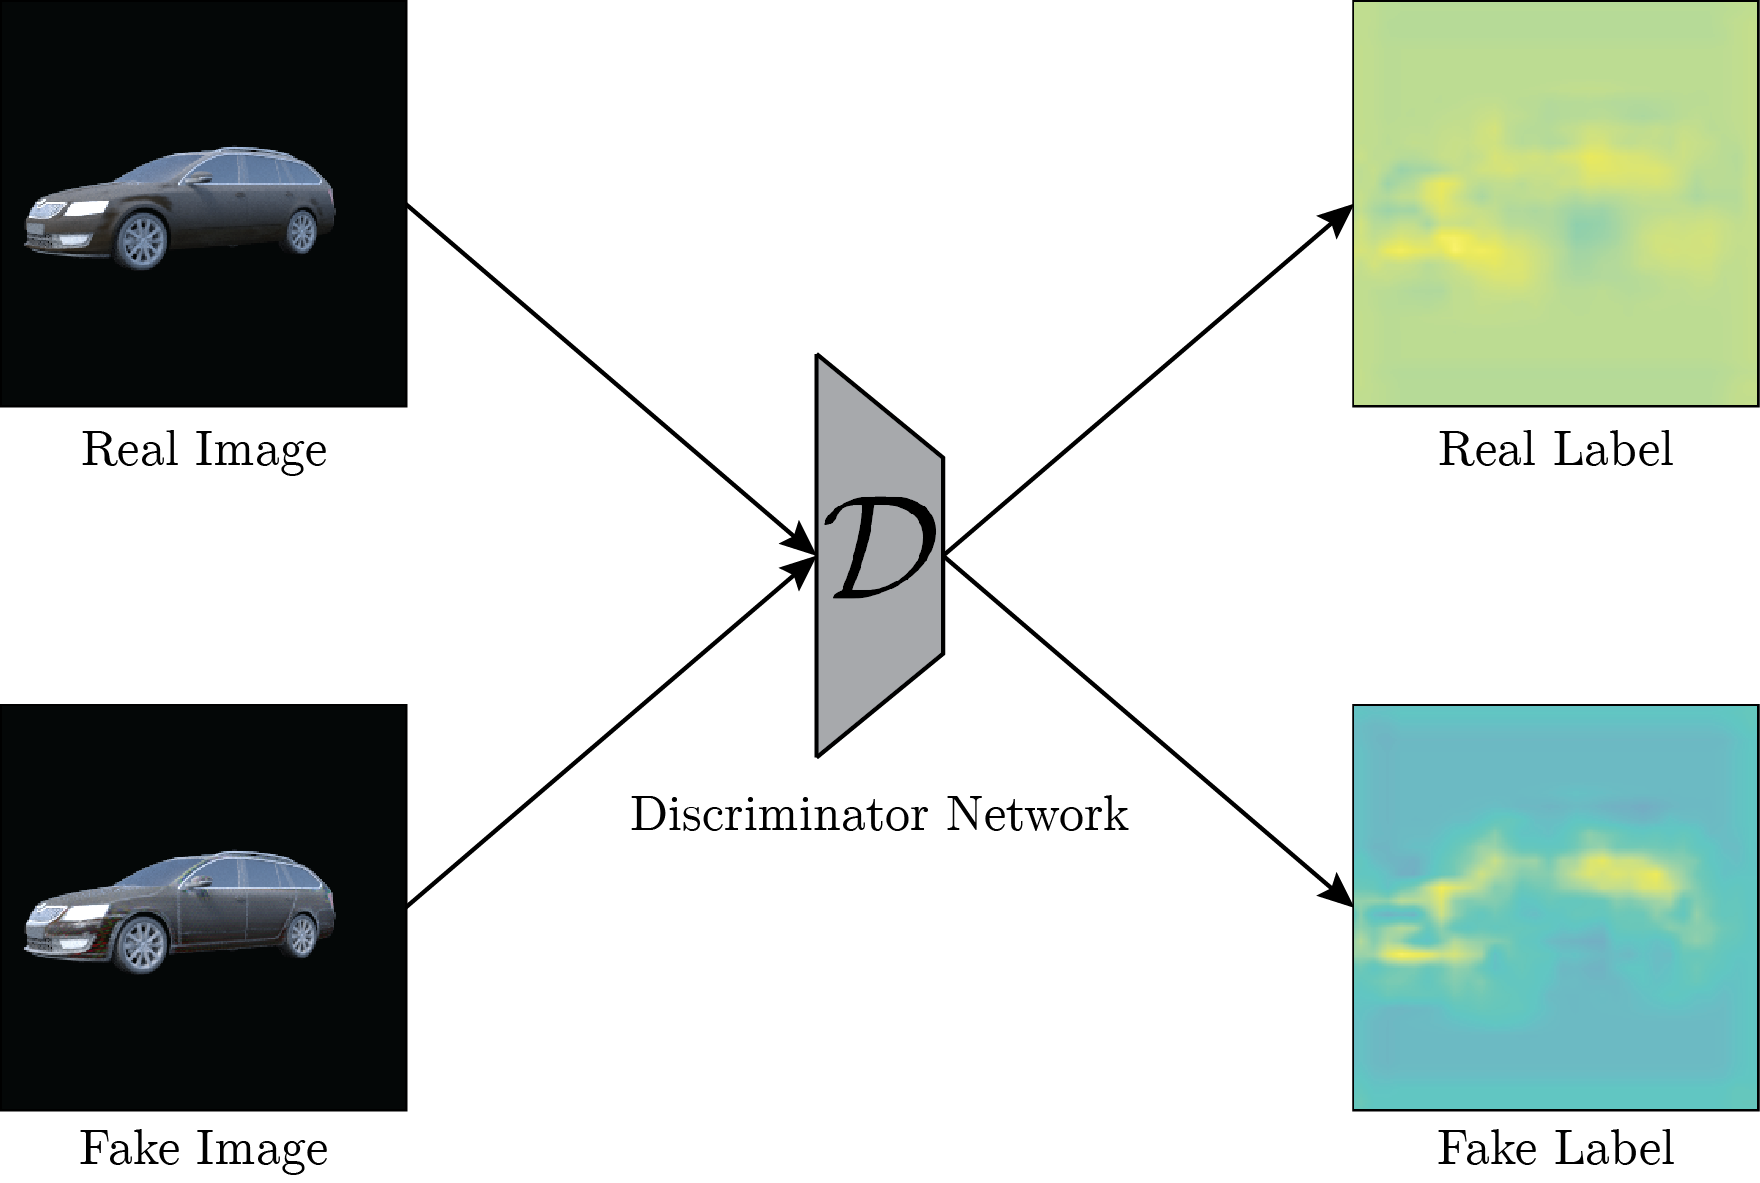
\includegraphics[width=.9\linewidth]{graphics/pipeline-2.png}
\end{figure}

\section{Differentiable Ray Tracing in Generative Models} \label{sec:diffrtgan}

The key contribution of this thesis is to frame this task as a learning problem and
incorporate the differentiable ray tracing function \cite{li2018differentiable} into the
learning process. We present a schematic of our models in Figure~\ref{fig:generator-pipeline}
and Figure ~\ref{fig:discriminator-pipeline}. We construct a convolutional neural network
$\mathcal{G}: \mathbf{x} \rightarrow \mathbf{y}$, which, given a car's surface geometry
$\mathbf{x}$, produces an albedo texture-map $\mathbf{y}$. We composit $\mathbf{y}$ onto the
base material of the car and render it using the differentiable ray tracer
$\mathcal{R}_\Phi: \mathbf{y} \rightarrow \mathbf{z}$ to obtain a rendered image $\mathbf{z}$
($\Phi$ is the parameter set which describes the scene). The combined model
$\mathcal{R}_\Phi \circ \mathcal{G}$ is fully differentiable, which allows us to train the
network weights of $\mathcal{G}$ using a loss computed from the rendered image
$\mathbf{z} = \mathcal{R}_\Phi \circ \mathcal{G}(\mathbf{x})$.

Although the render function is applicable for arbitrary network architectures, for the
scope of this thesis we train a generative adversarial network (GAN). Specifically, along with the generator $\mathcal{G}$,
our model also trains a discriminator $\mathcal{D}$ which learns to label a rendered image
of a car based on whether the albedo texture-map of the car was generated by $\mathcal{G}$
or by some ground-truth generator $\mathcal{G}_0$. $\mathcal{G}_0$ is a standard out-of-the-box
procedural surface weathering texture-map generator~\cite{bhandari2018procedural}.

\section{Model Input and Surface Parameterization}

\begin{figure}[ht]
    \centering
    \caption{The \emph{geometry buffer} is a mapping between UV-coordinates of the car
        triangle-mesh and     corresponding values of surface coordinates $\mathbf{p}$ and
        shading normals $\mathbf{n}$. We store these maps     as two RGB encoded images, with
        the three channels representing each dimension of $\mathbf{p}$ and $\mathbf{n}$
        respectively.}
    \label{fig:gbuffer}
    \vspace{0.2in}
    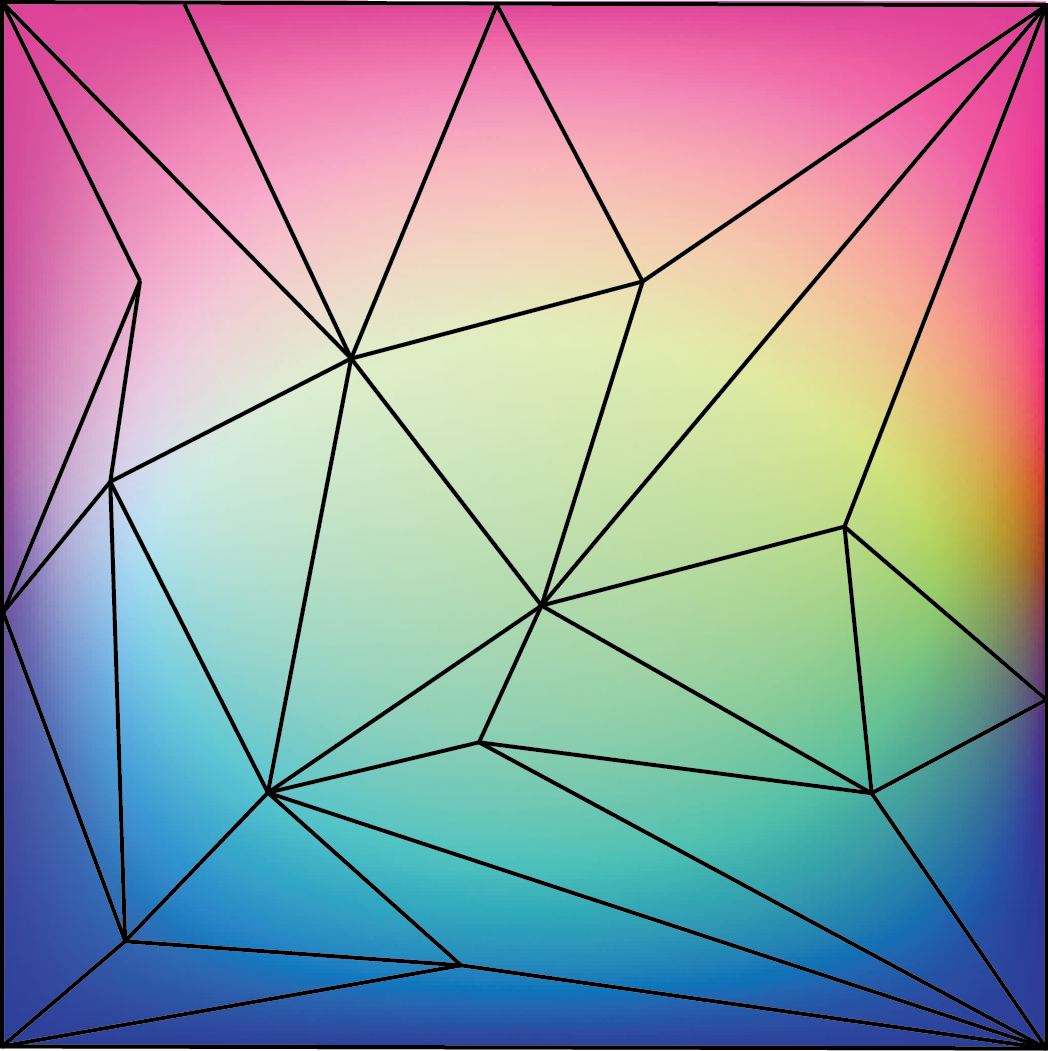
\includegraphics[width=.3\linewidth]{graphics/gbuffer.png}
\end{figure}

So far we've discussed how $\mathcal{G}$ takes as input the shape geometry of a car
$\mathbf{x}$ to produce a texture-map $\mathbf{y}$. For arbitrary generator models, the
surface geometry can be represented using any parameterization. However, in order to utilize
well tested CNN models such as \cite{johnson2016perceptual}, we require $\mathbf{x}$ to be in a
representation that is compatible with 2D convolutions.

To re-parameterize $\mathbf{x}$ into a 2D grid structure, we bake $\mathbf{x}$ onto the surface's
UV-embedding. I.e., given some UV-embededing for the input surface, for each UV-coordinate
$(u, v)$ we compute the surface's position vector $\mathbf{p}(u, v) \in \mathbb{R}^3$, and normal
vector $\mathbf{n}(u, v) \in \mathbb{R}^3$. Using $\mathbf{p}$ and $\mathbf{n}$, we form the
surface \emph{geometry buffer} $\mathbf{x} \in \mathbb{R}^6$ by concatenating the two vectors at
each UV-coordinate.

The convolutions which $\mathcal{G}$ applies to the \emph{geometry buffer} to generate the
surface albedo are similar to using 3D shape convolutions as proposed by Masci et al. 
\cite{masci2015shapenet} with the caveat of the convolution filter size changing depending on
the distortion of the UV-embedding. We provide more details about our choice of UV-embedding
as well as a discussion about desired specifications of the UV-embedding in Section
\ref{sec:uv-embedding}.
\chapter{Implementation} \label{ch:implementation}

\section{Surface UV-embedding} \label{sec:uv-embedding}

\begin{figure}[t]
    \centering
    \caption{Our implementation features a \emph{spherical UV-embedding} of the car surface.
        In this embedding we take the pair $(\theta, \phi)$ as shown in the figure, and
        scaled to unity to specify a planar coordinate which corresponds to the surface. We
        use this embedding to specify a generalizable UV-embedding across all our car models.}
    \label{fig:spherical}
    \vspace{0.2in}
    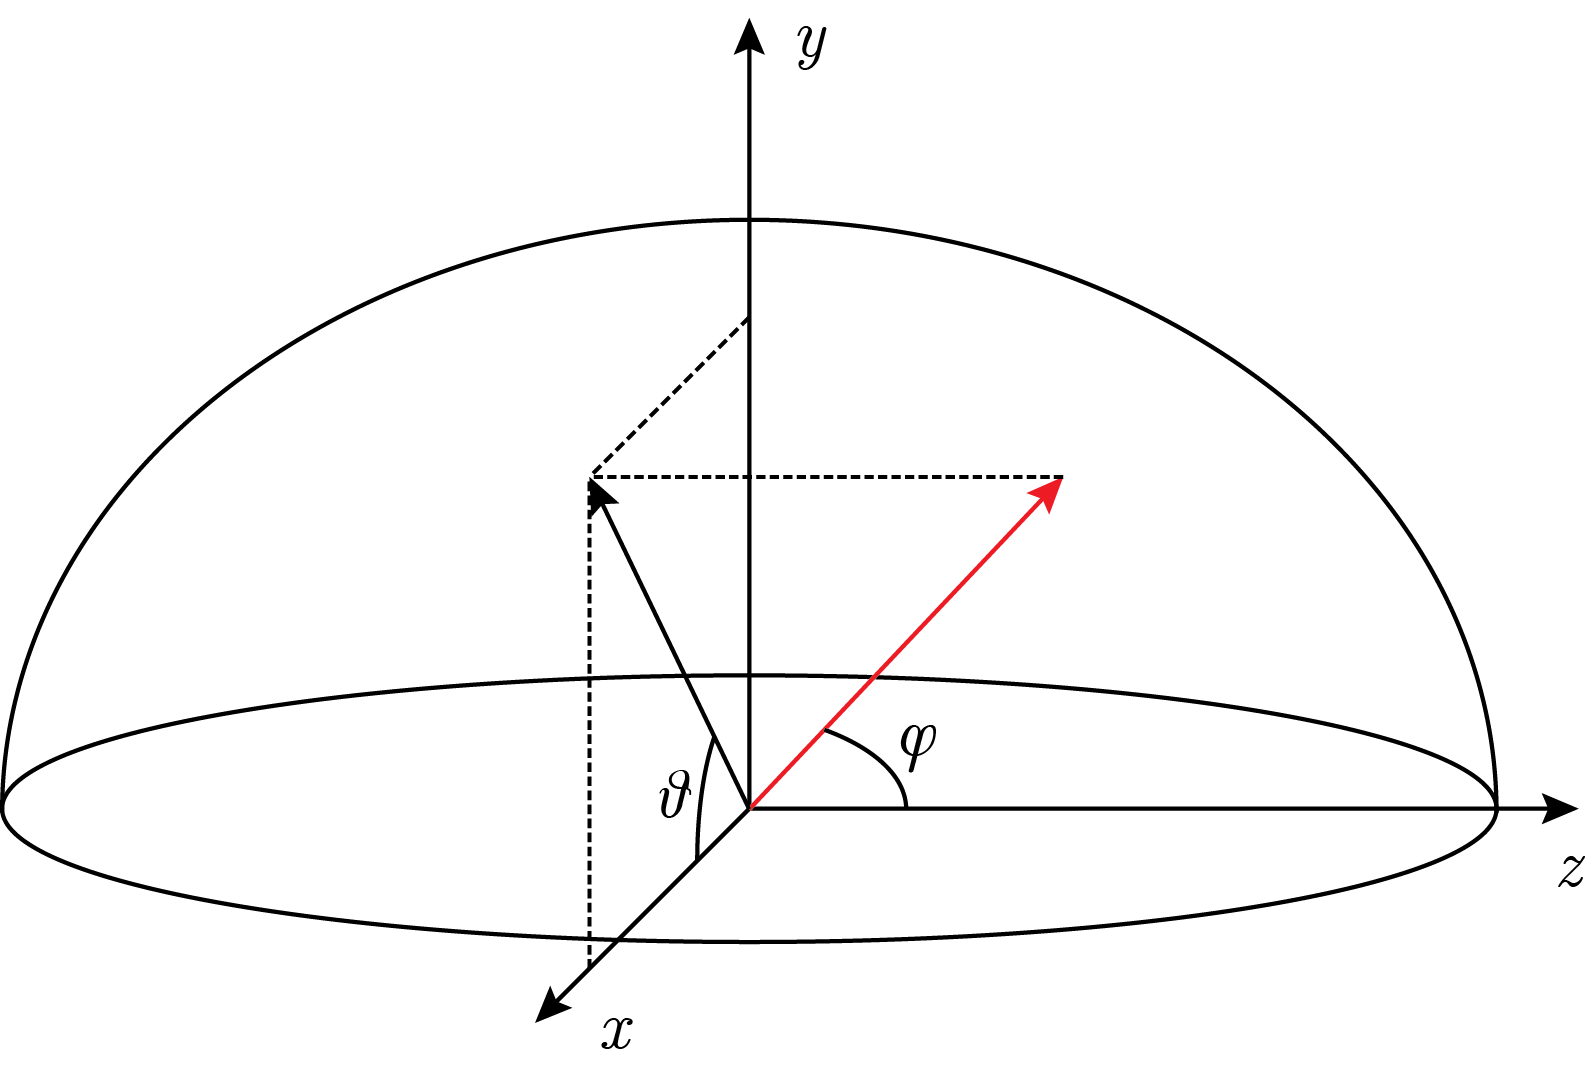
\includegraphics[width=.9\linewidth]{graphics/spherical.png}
\end{figure}

In Chapter~\ref{ch:method}, we briefly discussed that we construct the \emph{geometry buffer}
of a surface by using its UV-embedding. However, it is not obvious whether an arbitrary
UV-embedding can be applied for our model. Ideally, the model accepts any valid UV-embedding
and produces a corresponding albedo texture-map. However, there are several considerations
that make certain embeddings more useful than others. A good embedding should have the
following qualities:

\begin{itemize}
\renewcommand\labelitemi{--}
    \item Similarity of embeddings for similar surfaces is an important feature required for
        generalization capabilities of our model. I.e., if we feed in two similar car surfaces,
        we should expect similar UV-embeddings. This similarity allows the generator to
        learn to generate similar texture-maps for similar surfaces.
    \item General compactness of the embedding is also very important since we're restricted
        to using convolutions; any unassigned coordinates in the UV-embedding will take up space
        in the convolution input while not being used to produce the final texture-map.
    \item Conservation of surface connectivity in the UV-embedding ensures that operations that
        operate in local neighborhoods, such as convolutions, respect the surface connectivity.
        Otherwise, discontinuities caused by seams in the UV-embedding would create
        discontinuities along the seam when a generated texture-map is composited onto a surface.
    \item Low distortion is important due to the static size of the convolution filter used
        in the model. Applying a filter on a stretched out area of the embedding will
        shrink the effective size of the filter on the surface manifold and vice versa.
\end{itemize}

For our implementation, we normalize the UV-embeddings across all car surfaces using a
hemispherical parameterization. Given the $(x, y, z)$ coordinates of a point in the standard
Euclidean basis, we can compute its corresponding spherical coordinates $(r, \theta, \phi)$,
where the point is located a distance of $r$ away from the origin and oriented by the
azimuth angle $\theta$ and polar angle $\phi$. Using this change of coordinates, we construct
the hemispherical parameterization $(u, v) \in [0, 1]^2$ by discarding the radial distance $r$
and scaling $\theta$ and $\phi$ to a unit length. Since we're parameterizing a hemisphere,
(as opposed to a whole sphere) we scale $\theta$ by $\pi$ instead of $2 \pi$.

\begin{equation}
    (u, v) = (\theta / \pi, \phi / \pi)
\end{equation}

In general, the parameterization we described is not suitable for arbitrary shapes, especially
if the shape has overlapping points along a radial direction as these points will be assigned
to the same UV-coordinates. Fortunately, the roughly ellipsoid shape of car hulls allow us to
use this parameterization with minimal artifacts.

This parameterization is (1) similar between similar surfaces as long as the center
of each car model is standardized across models, (2) compact and roughly square since the
surface is roughly shaped like an ellipsoid, and (3) reflects the connectivity of the surface
well as our parameterization does not introduce any seams. Unfortunately, this parameterization
has high distortion near the poles of the parameterization. For the scope of this thesis we
do not address this issue, but we provide a discussion of a possible fix to this problem in
Section \ref{sec:distortion}.

\section{Dataset Generation}

We generate a synthetic dataset for model training using the ray tracer $\mathcal{R}_\Phi$
we described in Section \ref{sec:diffrtgan}, as well as a procedural surface weathering
texture-map generator $\mathcal{G}_0$~\cite{bhandari2018procedural}. In order to create a
diverse training dataset, we sample a random scene description $\Phi$ from a pool of car meshes,
base materials, environment maps, and camera parameters. We describe the distribution of assets
and their sampling strategies in more detail in Appendix \ref{app:system-overview}. Additionally,
we mark a subset of the materials as \emph{learnable} and composit the surface weathering
texture-map generated from $\mathcal{G}_0$ onto the base material of the surface using the
alpha-channel of the texture-map.

During training, each exemplar image from this dataset is loaded along with its corresponding
scene description $\Phi$ to aide in the training process. We evaluate our model $\mathcal{G}$
by comparing the fidelity of its results to $\mathcal{G}_0$. In Chapter~\ref{ch:experiment},
we discuss how the use of the scene description $\Phi$ of the training dataset affects the
performance of the model.

\section{Model Hyper-parameters}

\subsection{Network Architecture}

We adopt the network architecture choices by Zhou et al.'s model for non-stationary texture
synthesis~\cite{zhou2018non}. Our generator network is the
ResNet architecture by Johnson et al.~\cite{johnson2016perceptual}, featuring several
convolutions, followed by six residual blocks~\cite{he2016deep}, and several fractionally
strided convolutions. Our discriminator network is the PatchGAN architecture~\cite{isola2017image}.

\subsection{Loss Function}

Empirical results show that training with the Wasserstein GAN loss with gradient penalty as
proposed by Gulrajani et al.~\cite{gulrajani2017improved} produce the best results with the
fastest convergence rates, compared to the vanilla GAN loss~\cite{goodfellow2014generative}
and the LSGAN loss~\cite{mao2017least}. We present a comparison between these models in
Chapter~\ref{ch:experiment}.

\subsection{Training Process} \label{training-process}

The differentiable ray tracer~\cite{li2018differentiable} is a computation and memory
intensive operation, even when run on a GPU. Our experiments show that rendering an image
with resolution of $256 \times 256$, scene complexity of $\mathtt{\sim} 1,000,000$ vertices,
and Monte-Carlo sub-sampling rate of $200$ per pixel, takes $\mathtt{\sim} 0.3$ seconds in
the forward direction and $\mathtt{\sim} 9.0$ seconds in the backward direction (i.e.
computing the derivative); running multiple render operations in parallel on the GPU further
increases this runtime. We found that using a smaller Monte-Carlo sub-sampling rate in the
backward direction gives us a more reasonable runtime of $\mathtt{\sim}  0.9$ seconds at the cost
of accuracy of the computed derivatives.

Still, coupled with the large memory footprint the operation requires to store the scene
description and relevant metadata needed for derivative computations, training the model
with a large batch size is unfeasible unless we have a dedicated cluster of GPUs with
synchronized training. Due to these limitations, we conducted all experiments using batch size
of $1$ on a single GPU. \cite{zhu2017unpaired} shows that training GAN architectures with a batch
size of $1$ produces good results.

\chapter{Experiments} \label{ch:experiment}

In this section, we present the experiments we conducted for our model along with the
corresponding results for each experiment.

\section{Training Results} \label{sec:training-results}

We found that the model fails to learn the target texture accurately when the distribution
of the set of scene descriptions used for generating the dataset does not match the set of
scene descriptions used at runtime during training. We attribute this failure mode to two
primary causes.

\begin{figure}
    \centering
    \caption{We present our results side-by-side with the ground truth albedo as generated by
    a procedural dirt texture generator $\mathcal{G}_0$. The dataset this model was trained on
    contains images of cars rendered only from one side with a constant elevation angle. This
    causes the model to not learn patches that weren't visible in the whole dataset.}
    \label{fig:results-albedo}
    \vspace{0.2in}
    \begin{subfigure}[t]{0.4\linewidth}
        \centering
        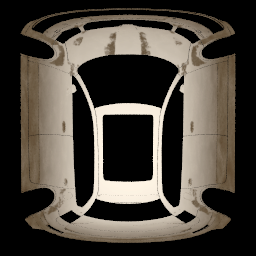
\includegraphics[width=\linewidth]{graphics/results_0_albedo.png}
        \caption{Target albedo}
    \end{subfigure}
    \begin{subfigure}[t]{0.4\linewidth}
        \centering
        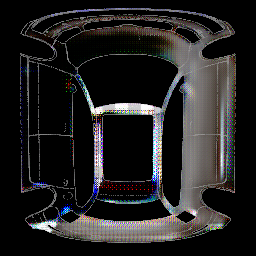
\includegraphics[width=\linewidth]{graphics/results_1_albedo.png}
        \caption{Model output}
    \end{subfigure}
\end{figure}

\begin{figure}[t]
    \centering
    \caption{We render the albedo-maps from Figure~\ref{fig:results-albedo} onto its corresponding
    car mesh and compare to the ground truth images.}
    \label{fig:results}
    \vspace{0.2in}
    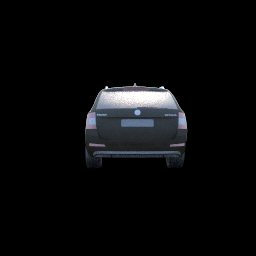
\includegraphics[width=.19\linewidth]{graphics/results_1_target.png}
    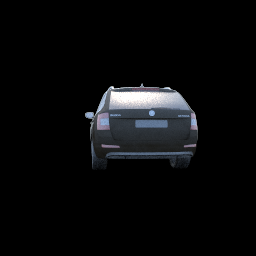
\includegraphics[width=.19\linewidth]{graphics/results_2_target.png}
    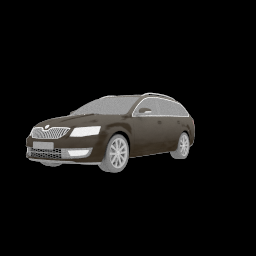
\includegraphics[width=.19\linewidth]{graphics/results_3_target.png}
    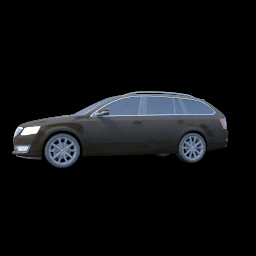
\includegraphics[width=.19\linewidth]{graphics/results_4_target.png}
    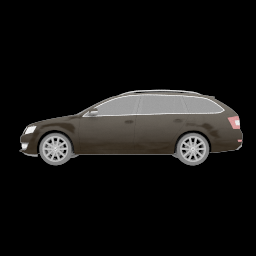
\includegraphics[width=.19\linewidth]{graphics/results_5_target.png}
    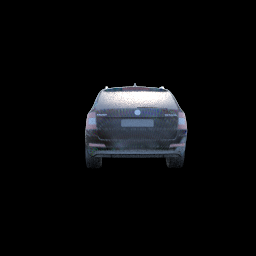
\includegraphics[width=.19\linewidth]{graphics/results_1_model.png}
    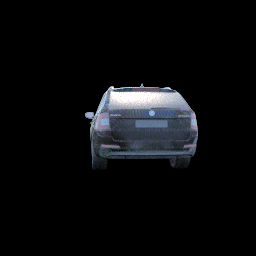
\includegraphics[width=.19\linewidth]{graphics/results_2_model.png}
    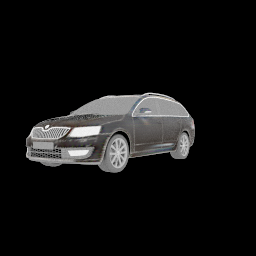
\includegraphics[width=.19\linewidth]{graphics/results_3_model.png}
    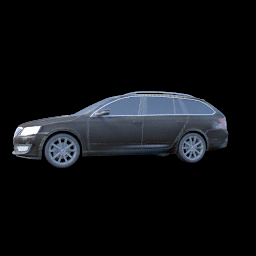
\includegraphics[width=.19\linewidth]{graphics/results_4_model.png}
    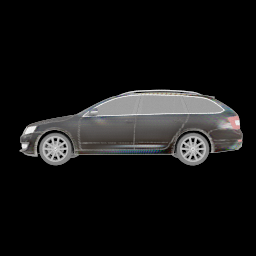
\includegraphics[width=.19\linewidth]{graphics/results_5_model.png}
\end{figure}

\begin{itemize}
\renewcommand\labelitemi{--}
    \item The discriminator learns to distinguish between the real and fake images using
        the discrepancy in the statistics of the scene description that is used to render it
        instead of using the generator output. We refer to this failure mode as discriminator
        \emph{mode collapse}.
    \item A batch size of $1$ prevents the model from passing useful gradients to the network
        weights due to lack of feature overlap between real and fake images at each iteration.
\end{itemize}

In order to address both of these issues, we elect to train the network by specifying the
scene description for each image using the scene description of the training images: at each
training iteration of the discriminator, an output from the generator is computed and applied
to the same scene as in the training image. The discriminator computes the GAN-loss on this
pair of real and fake images. Throughout this training procedure, the only difference the
discriminator observes between the pair of fake and real input images is the texture applied
to the cars.

This approach allows us to determine a baseline for whether our model is capable of learning
the target texture provided no ambiguity on what the discriminator can use to distinguish
real images from fake images.

\section{Ablation Study}

As mentioned in the previous section, our model does not train well unless the input image
scene description is shared between the real and fake images. We recognize that this
constraint prevents us from training our model on anything beyond the synthetic dataset we
generated for training purposes. If we hope to generalize our model for real image datasets
in the future, determining the model's robustness to non-matching scene-descriptions is
crucial. In this section, we present results from training our model after relaxing the
"matching scene description" constraint in a variety of controlled situations as a measure
of stress-testing our model's robustness.

\subsection{Camera Pose Distribution}

\begin{figure}
    \centering
    \caption{Increasing the noise $\epsilon$ in the pose estimation during training
        preserves the quality of the textures learned by the model. However, if the
        model and dataset pose distributions are non-overlapping, the discriminator
        experiences \emph{mode collapse}.}
    \label{fig:pose-vary-1}
    \vspace{0.2in}
    \begin{subfigure}[t]{0.19\linewidth}
        \centering
      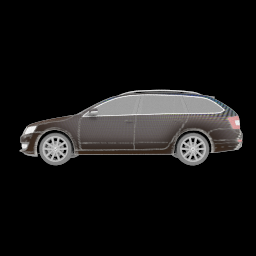
\includegraphics[width=\linewidth]{graphics/pose_1.png}
        \caption{$\epsilon < 1^\circ$}
    \end{subfigure}
    \begin{subfigure}[t]{0.19\linewidth}
        \centering
       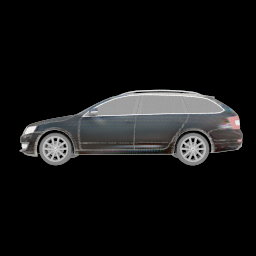
\includegraphics[width=\linewidth]{graphics/pose_2.png}
        \caption{$\epsilon < 2^\circ$}
    \end{subfigure}
    \begin{subfigure}[t]{0.19\linewidth}
        \centering
       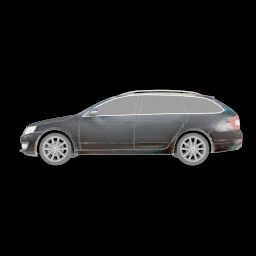
\includegraphics[width=\linewidth]{graphics/pose_5.png}
        \caption{$\epsilon < 5^\circ$}
    \end{subfigure}
    \begin{subfigure}[t]{0.19\linewidth}
        \centering
        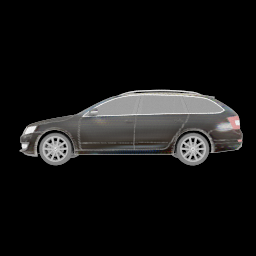
\includegraphics[width=\linewidth]{graphics/pose_10.png}
        \caption{$\epsilon < 10^\circ$}
    \end{subfigure}
    \begin{subfigure}[t]{0.19\linewidth}
        \centering
        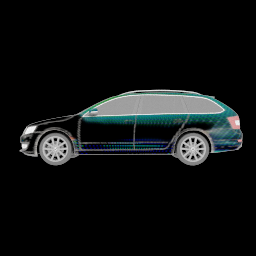
\includegraphics[width=\linewidth]{graphics/pose_diff.png}
        \caption{No overlap}
    \end{subfigure}
\end{figure}

We discussed the technical limitations that require us to train with a batch size of $1$
in Section \ref{training-process}. As a result we are not able to benefit from gradient averaging
used in deep learning models which decrease the volatility of the gradient at each iteration. If
at each iteration, the discriminator observes vastly different fake and real images, the
discriminator's task becomes more complex as it will have to learn to ignore the pose variation
of the cars before learning to label images using the texture observed on the car surfaces.

However, having perfect estimation of the camera pose from a real image is not realistic. At
best, we can get a noisy estimate of the camera pose. To investigate how much noise in camera
pose estimation the model can tolerate and what the effect is on model convergence speed and
the quality of the learned textures, we conduct several experiments where we perturb the camera
pose loaded from the training image scene by some random uniform noise. The results for this
experiments are shown in Figure~\ref{fig:pose-vary-1}. The figure shows that errors of up to 10
degrees in the pose estimation still allow the model to learn a reasonable texture-map. However,
the training time for the model increases as the noise increases.

In order to confirm our assumptions stated earlier, we experiment with a setup where the
distribution of the camera poses between the real and fake images is completely independent and
non-overlapping. If our assumption about the discriminator's \emph{mode collapse} as explained in
Section \ref{sec:training-results} is correct, this model should fail to learn a reasonable
texture-map. Unsurprisingly, this model does not learn a reasonable texture-map as shown in
Figure~\ref{fig:pose-vary-1}, likely because the discriminator learns the difference in camera
pose distributions between the real and fake image sets.

\subsection{Environment Map Distribution}

\begin{figure}
    \centering
    \caption{Varying the environment map distribution affects the quality of the outputs of our
        model. If we train a network with non-matching environment maps sampled from
        the training distribution, we learn a reasonable texture as shown in
        Figure~\ref{fig:pose-vary-sim}. Unfortunately, using environment maps sampled from a
        different distribution leads to \emph{mode collapse}.}
    \label{fig:pose-vary-1}
    \vspace{0.2in}
    \begin{subfigure}[t]{0.24\linewidth}
        \centering
        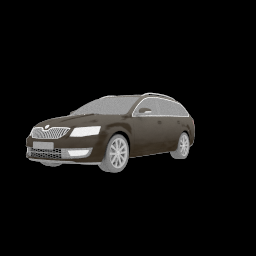
\includegraphics[width=\linewidth]{graphics/envmap_target.png}
        \caption{Target Image}
    \end{subfigure}
    \begin{subfigure}[t]{0.24\linewidth}
        \centering
       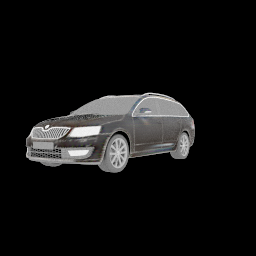
\includegraphics[width=\linewidth]{graphics/results_3_model.png}
        \caption{Same dist, match}
    \end{subfigure}
    \begin{subfigure}[t]{0.24\linewidth}
        \centering
        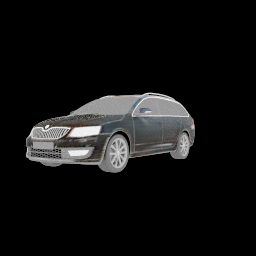
\includegraphics[width=\linewidth]{graphics/envmap_sim.png}
        \caption{Same dist, no match}
        \label{fig:pose-vary-sim}
    \end{subfigure}
    \begin{subfigure}[t]{0.24\linewidth}
        \centering
        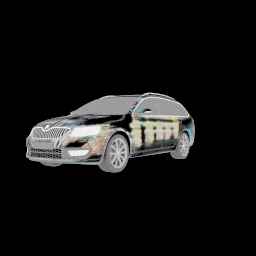
\includegraphics[width=\linewidth]{graphics/envmap_diff.png}
        \caption{Different dist, no match}
    \end{subfigure}
\end{figure}

The overall brightness, contrast, and white balance of a rendered image is heavily affected
by the lighting parameters of the scene. We observe that the choice of environment map
distributions has the highest amount of effect on the network's ability to learn the target
texture.

For the environment map ablation study, we experiment with two general setups for which we
report our findings.

\subsubsection{Non-matching samples drawn from the same distribution}

At each iteration, we render the fake image by randomly sampling an environment map
configuration that does not match the configuration loaded from the scene description of the
real image. However, we sample the configuration from the same distribution as the real image
dataset. Doing so allows us to check whether there are any effects other than discriminator
\emph{mode collapse}. The results of this experiment show that the model successfully learns
the target texture, albeit with a slower convergence rate, which is expected.

\subsubsection{Samples drawn from a different distribution}

In this setup, we draw the samples of environment map configurations for the fake and real
images from a mutually exclusive distribution; each set is rendered using completely different
environment maps. Unfortunately, in this experiment the model fails to converge on a realistic
surface texture-map generator. This result is likely due to \emph{mode collapse}.

The inability to learn a texture-map due to inaccuracy of the environment map makes it difficult
for us to easily extend our model to train on real images. Unless we have a good estimation
of the set of environment maps used in the dataset, the model will fail to converge on real images.

\section{GAN Loss function}

Different GAN loss functions have vastly different results when trained for our model.
Figure~\ref{fig:gan-results} shows the comparative results between the convergence speed and
resultant textures between vanilla GAN loss, WGAN loss with gradient penalty, and LSGAN loss
functions respectively. The WGAN with gradient penalty shows the best results visually, while the
LSGAN model fails to learn a reasonable texture-map.

\begin{figure}
    \centering
    \caption{Different GAN loss functions produce different results when training our model. From
        left to right, we show our results for vanilla GAN, WGAN w/ gradient penalty, and LSGAN.
        The LSGAN model falls into \emph{mode collapse}.}
    \label{fig:gan-results}
    \vspace{0.2in}
    \begin{subfigure}[t]{0.3\linewidth}
        \centering
       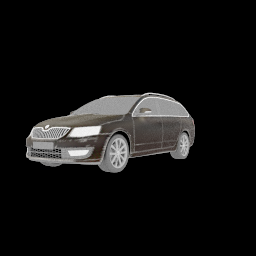
\includegraphics[width=\linewidth]{graphics/gan_vanilla.png}
        \caption{Vanilla GAN}
    \end{subfigure}
    \begin{subfigure}[t]{0.3\linewidth}
        \centering
      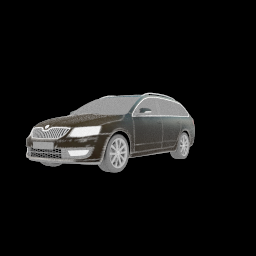
\includegraphics[width=\linewidth]{graphics/gan_wgangp.png}
        \caption{WGAN w/ gp}
    \end{subfigure}
    \begin{subfigure}[t]{0.3\linewidth}
        \centering
      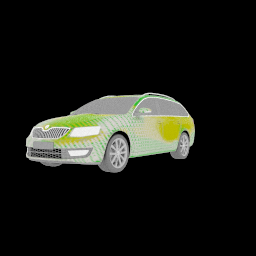
\includegraphics[width=\linewidth]{graphics/gan_lsgan.png}
        \caption{LSGAN}
    \end{subfigure}
\end{figure}
\chapter{Discussion and Further Work}

This thesis presents promising results for a potential application of differentiable ray
tracing~\cite{li2018differentiable} in deep learning models. Our results in
Chapter~\ref{ch:experiment} demonstrate the extent of our model's generative ability while also
outlining the limitations of our technique. In this section, we discuss the source of these
limitations and suggest potential improvements to be explored as further work.

\section{Distortion in mesh parameterization} \label{sec:distortion}

In Section \ref{sec:uv-embedding}, we justified a simple UV-embedding which utilized the
spherical parameterization of the points on the surface while noting the poor distortion
qualities of the embedding. For the scope of this thesis, we focused on improving the
learning task, and were not able to address the distortion artifacts appropriately. As
future work, it is more desirable to use a better UV-embedding parameterization that
minimizes surface distortion, such as Sander et al.'s solution of running an optimization
to minimize the stretch metric of the embedding~\cite{sander2001texture},

\section{Generalizing the model for real images}

Although the ultimate goal of our model is to learn texture-maps of surface weathering based
on exemplar images of real cars, we found directly training GANs on a dataset of real
images to be difficult due to volatility of the model to \emph{mode collapse}. There are many
details of real scenes have which are very difficult to emulate in a 3D scene and vice versa.

An example of a fundamental difference between ray traced images and real scene images is
Monte-Carlo noise artifacts produced in ray traced images. Monte-Carlo noise is caused by the
stochastic nature of Monte-Carlo sampling and leads to noisy images as shown in Figure
\ref{fig:monte-carlo}. Although this noise decreases with higher MC sampling rates, the SNR improves
roughly with $O(n^{1/2})$ where $n$ is the sampling rate. Therefore, computationally, it
becomes infeasible to keep increasing the samples we use per pixel. However, unless the
dataset has noticeably less Monte-Carlo noise compared to the input dataset, the discriminator
learns to distinguish the fake and real images using the noise profile of its input image in a
similar fashion as we showed in Chapter~\ref{ch:experiment}.

\begin{figure}
    \centering
    \caption{Monte-Carlo sub-sampling per pixel has a huge effect on the resultant render.
        Training the model using a low Monte-Carlo sub-sampling rate causes the discriminator
        to \emph{mode collapse} due to the discrepancy in render quality.}
    \label{fig:monte-carlo}
    \vspace{0.2in}
    \begin{subfigure}[t]{0.32\linewidth}
        \centering
        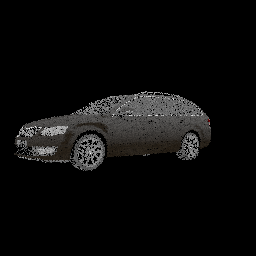
\includegraphics[width=\linewidth]{graphics/mc1.png}
        \caption{1 sub-sample}
    \end{subfigure}
    \begin{subfigure}[t]{0.32\linewidth}
        \centering
        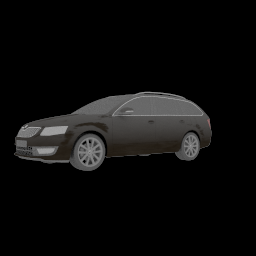
\includegraphics[width=\linewidth]{graphics/mc200.png}
        \caption{200 sub-samples}
    \end{subfigure}
\end{figure}

This artifact is only one of many difficulties associated with the problem of extending our
model to train on real images. However, our current hypothesis is that the discriminator uses
the most easily learnable feature to distinguish between real and fake images. If we keep
eliminating the most easily learnable feature that is not the dirt texture on the surface of the
car, we hope that the discriminator will eventually be forced to learn to distinguish clean
cars from dirty ones.

\section{Differentiable ray tracing in deep learning applications}

This thesis primarily focused on generating simple diffuse textures. But our general method
applies to learning arbitrary scene description parameters using deep learning models.
Improving the surface shader complexity of our model, such as adding learnable specular
components and normal maps, would add more expressiveness to the output textures. Furthermore,
we can also attempt to train a model which learns shapes of surfaces in 3D using images of
these shapes. Regardless of the specific application in mind, we hope that our work can be a
good baseline for deep learning models featuring differentiable ray tracing in future research.

\appendix
\chapter{System Overview} \label{app:system-overview}

We implemented the model using the auto-differentiation library PyTorch~\cite{paszke2017automatic}.
Most of our code was written in Python, and several auxiliary mesh processing scripts use the Blender
Python API. Our pipeline features:
%
\begin{itemize}
\renewcommand\labelitemi{--}
    \item a GAN model architecture featuring the differentiable ray tracer~\cite{li2018differentiable}
    \item a dataset generation pipeline which uses the same ray tracer as our model
    \item auxilliary input pre-processing scripts.
\end{itemize}

Our codebase structure is based off of the PyTorch implementation by Zhu et al.~\cite{zhu2017unpaired},
and Isola et al.~\cite{isola2017image}. For features of the codebase such as network implementations, GAN
model setup, and training scripts, we refer to their github repository at
\url{https://github.com/junyanz/pytorch-CycleGAN-and-pix2pix}. In this chapter, we describe the modules of
the codebase that relate to the differentiable rendering and dataset generation process.

\section{Render Utilities}

The differentiable ray tracer~\cite{li2018differentiable} presents an generic interface that is not
necessarily purposed for the PyTorch neural network module. We add a wrapper to the ray tracer so that
we can add the render operation into a PyTorch neural network as a \texttt{RenderLayer}. As
described in Chapter~\ref{ch:method}, the \texttt{RenderLayer} takes as input the scene description $\Phi$
and a texture-map to render an image. The scene description $\Phi$ is specified by the ray tracer
primitives, and the texture-map is a $(\text{Height} \times \text{Width} \times \text{Channel})$ PyTorch
Tensor object. The last dimension of the Tensor encodes the \texttt{RGBA} values for each pixel.

Native PyTorch neural network modules are laid out in $(\text{Batch} \times \text{Channel} \times
\text{Height} \times \text{Width})$ order. In order to convert between these formats, we implement custom
network layers that handle the conversion.

Loading large files containing car triangle-meshes and swapping them out at each iteration slows down the
rendering process significantly. Additionally, since we're dealing with over 100 triangle-meshes during
training, we cannot load all the car models into GPU memory simultaneously. To mitigate these issues we
pre-process all elements in the scene description $\Phi$ by loading them into memory and storing them to
disk in its pickled format.

\section{Dataset Generation}

When we generate a dataset for training, our goal is to have a high degree of control for the output
datasets. In Chapter~\ref{ch:experiment} we presented results from training our model on datasets with
different distributions of the scene description, $\Phi$. We implemented a \texttt{ConfigSampler} that
allows us to specify what kind of distributions to sample $\Phi$ from. When generating each image of the
new dataset, the \texttt{ConfigSampler} samples $\Phi$ from the specified distribution and renders an image
specified by $\Phi$ and stores $\Phi$ to disk. During training, we use the ground truth $\Phi$, to generate
a similar scene description $\Phi_{training}$. This setup allows us to test the resilience of our model
with respect to errors introduced to $\Phi$.

\section{Auxiliary Scripts}

We provide several auxiliary scripts for
\begin{itemize}
\renewcommand\labelitemi{--}
    \item adding a spherical parameterization for meshes
    \item generating the \emph{geometry buffer} for a spherically parametrized mesh
    \item generating dirt texture-maps for a car mesh using the Blender API.
\end{itemize}
%% This defines the bibliography file (main.bib) and the bibliography style.
%% If you want to create a bibliography file by hand, change the contents of
%% this file to a `thebibliography' environment.  For more information 
%% see section 4.3 of the LaTeX manual.
\begin{singlespace}
\bibliography{main}
\bibliographystyle{plain}
\end{singlespace}

\end{document}

